%!TEX root = ../thesis_polimi.tex

\chapter{Botnets} % (fold)
\label{chap:botnets}
\start{A}{botnet} is a network of compromised machines, remotely controlled
by the \emph{botmaster}. These malicious infrastructures are deployed by the
attackers for profit, and the more machines are compromised, the more powerful the
infrastructure, the more profitable the business. In the last years we
have witnessed an aggressive spread of this phenomenon that \emph{defenders}
from both the industry and the academia are striving to mitigate. In this
chapter we will tackle the different aspects of botnets in order to give
a brief yet insightful overview of this threat.

\paragraph{Chapter Organization} The remainder of the chapter is organized in
the following fashion:
\begin{itemize}
    \item in Section~\ref{sec:what_is_a_botnet} we explain what is a botnet;
    \item in Section~\ref{sec:botnet_topologies} we explain the different
        topologies a botnet can feature;
    \item in Section~\ref{sec:botnets_communications} we explain how botnet's
        hosts communicate;
    \item in Section~\ref{sec:domain_generation_algorithms} we deeper analyze
        a certain way to communicate, on which we focus in
        \thesystem;
    \item in Section~\ref{sec:botnet_countermeasures} we overview the possible
        techniques to mitigate a botnet;
    \item in Section~\ref{sec:botnets_a_modern_threat} we provide two case
        studies to better  explain why this phenomenon is a serious and expanding
        threat.
\end{itemize}


\newpage

%-----------------------------------------------------------------------------%
% Section: What is a botnet?
%-----------------------------------------------------------------------------%
\section{What is a botnet?} % (fold)
\label{sec:what_is_a_botnet}
\sectionstart{A}{botnet} is a network of compromised machines called \emph{bots}
or \emph{zombies} under the remote control of a human operator called
\emph{botmaster}~\cite{feily2009}.


The \emph{bot} is the piece of software that infects and compromises the machines.
The infection is carried out through a variety of so-called \emph{distribution channels}, which vary from compromised websites that serve malware via drive-by
mechanisms to phishing.
Once infected, the machine will continue to work as nothing changed to the eyes
of the legitimate user, while it is now capable of executing malicious
activities on the behalf of the \emph{botmaster}, who will employ a Command and
Control Server (C\&C) to dispatch orders to and gather information from
the \emph{zombies}. What is the nature of these criminal activities are
addressed in the next paragraphs.

\begin{figure}[!htp]
\centering
\begin{tikzpicture}[scale=0.6, every node/.style={transform shape}]
    \node [label=below:C\&C Server](CANDC) {
\includegraphics{server.eps}};
    \node [label=below:Botmaster](MASTER) [left=2cm of CANDC]{
\includegraphics{attacker.eps}};
    \node [label=below:Zombie](LAPTOP) [above right = 3cm of CANDC] {
\includegraphics{laptop_infected}};
    \node [label=below:Zombie](LAPTOP_2) [right = 3cm of CANDC] {
\includegraphics{nexus_infected.eps}};
    \node [label=below:Zombie](LAPTOP_3) [below right = 3cm of CANDC] {
\includegraphics{desktop_infected}};

    \path[arrow, <->]
        (CANDC) edge (LAPTOP)
        (CANDC) edge (LAPTOP_2)
        (CANDC) edge (LAPTOP_3);

    \path[arrow]
        (MASTER) edge (CANDC);
\end{tikzpicture}
\caption{An example of a botnet.}
\label{fig:botnet_example}
\end{figure}

\subsection{Botnet Purposes} % (fold)
\label{sub:purposes}
The main purpose of a malicious botmaster is to recruit as many \emph{zombies} as possible
in his army, as any botnet activity augments its effectiveness by the number
of \emph{bots} involved. In the following of this section we depict \emph{a few}
scenarios of malicious activities carried out employing this type of infrastructure.

\paragraph{Information Gathering} Botnets of this type aim at stealing personal
data of various kind from the infected machines. \texttt{Torpig} for instance,
which we shall further analyze in Section~\ref{sub:torpig}, was crafted with the precise
intention of stealing financial accounts credentials and credit or debit card
numbers. Beside personal data, we can think of a scenario where the infected
machines reside inside a corporate network. In this case the targets would be
trade secrets, as intellectual properties or management plans.

\paragraph{Distributed Computing} The network of infected machines can be
leveraged to perform computing-intensive tasks. One of the most interesting
ones is Bitcoin mining: Cybercriminals aim at creating a botnet of infected machines forced to perform complex calculations to earn them money, putting the
machines under heavy CPU and GPU load~\cite{spagnuolo2013}.
\texttt{Trojan.Coinbitminer} is an example of this type of
malware\footnote{\url{http://www.symantec.com/security_response/writeup.jsp?docid=2011-072002-1302-99}}.

\paragraph{Spamming} Spamming is one of the most known malicious activities.
Spamming botnets are used to send out a high volume of e-mails with various purposes, amongst which
we find malware spreading as an e-mail attachment (the \texttt{Cryptolocker} malicious binary was spread in this
fashion in its early versions, see Section~\ref{sub:cryptolocker}), frauds, XSS attacks and
advertisement of malicious services, basically using the bots as mail transfer agents without the victims noticing. It is not easy to set up and keep active
such an infrastructure, as spam sources get blacklisted and the messages are no
longer delivered. By employing a \emph{distributed} rather than \emph{centralized}
message dispatching servers architecture, the attackers aim at and succeed in
circumventing this obstacle.

\paragraph{Distribute Denial of Service} Distribute Denial of Service (DDoS)
is an attack where a machine receives an excessive amount of requests. To overcome
the overwhelming volume of incoming traffic, usually the machine interrupts its
services. This results in economic loss, especially when the company business
heavily depends on the offered service online availability. In this case the bots
are commanded by the botmaster to send an excessive amount of requests to the
targeted machine.

\paragraph{Malware Diffusion} Once the \emph{bot} program infects a machine,
it can be used to install \emph{further} malware. An example of this behavior
comes from the recent Cryptolocker \emph{ransomware}: Its primary vector of
infection was the \texttt{Zeus Gameover} P2P botnet, beside being spread via
e-mail spamming.
% subsection purposes (end)

\subsection*{Summary} % (fold)
\label{sub:what_summary}
In this section we have defined \emph{what} is a botnet and discussed \emph{why}
an attacker would struggle to create this type of networks. In the next section
we want to present the different topologies a botnet can be structured into and
explain why we chose to target the \emph{centralized} architecture.

% subsection summary (end)
% section what_is_a_botnet (end)


%-----------------------------------------------------------------------------%
% Botnet Topologies
%-----------------------------------------------------------------------------%
\section{Botnet Topologies} % (fold)
\label{sec:botnet_topologies}
\sectionstart{D}{ifferent} botnet topologies, imply different benefits and
weaknesses. Our study will focus on the centralized architecture, as it is
the most spread, even though recent reports~\cite{enisa2013} indicate a rise
in the P2P topology. Remarkably, certain P2P botnets automatically fall back to centralized topologies in case of failures to avoid  starvation of the bots.

\subsection{Centralized} % (fold)
\label{sub:centralized}
This topology reflects the classic  and well-established \emph{client-server}
pattern.
The bots communicate directly with the botmaster~\cite{schiavoni2013}, which forwards messages between clients~\cite{bailey2009}. This technique
guarantees \emph{i)} low latency and \emph{ii)} control over the packet delivery.
On the other hand its weaknesses are caused by \emph{i)} a single point of
failure, if the C\&C is compromised the whole botnet is, and \emph{ii)} are
easier to detect, since many clients connect to the same point~\cite{bailey2009}.
% subsection centralized (end)

\subsection{P2P} % (fold)
\label{ssub:p2p}
The main advantage in employing a P2P technology consists of a much more robust
and resilient infrastructure, as we do not have anymore a single point of
failure, but each bot is responsible of broadcasting the message received to
the other \emph{zombies}.
However, the design of P2P systems are more complex and there are typically no
guarantees on message delivery or latency~\cite{bailey2009}.
% subsection p2p (end)

\subsection{Unstructured} % (fold)
\label{sub:unstructured}
This is another way to design a botnet, featuring \emph{zombies} that are
completely agnostic with respect to the same botnet they belong to. Whenever
they need to send a message to the infected network, they encrypt it, randomly
scan the Internet and pass along the message when they detect another bot.
Even though the design is quite simple, it would not be able to guarantee the
actual deliver and it would also be prone to extremely high latencies.
% subsection unstructured (end)

\subsection*{Summary} % (fold)
\label{sub:topology_summary}
We have presented three different topologies a botnet can be structured into and
explained that we chose the \emph{centralized} architecture as it is the most
used by the attackers. Now we want to understand how the \emph{zombies}
communicate with the \emph{botmaster}.

% subsection summary (end)
% section botnet_topologies (end)


%-----------------------------------------------------------------------------%
% Botnets Communications Systems
%-----------------------------------------------------------------------------%
\section{Communication Systems of DNS-based Botnets} % (fold)
\label{sec:botnets_communications}
\sectionstart{E}{very} distributed network of machines must be equipped with
a communication protocol, as communication intra hosts is a defining feature
of these architectures. Before starting the exchange of malicious commands, the
\emph{bots} and the \emph{botmaster} must establish a connection. In centralized botnets, this happens through the C\&C Server
in the so called \emph{rallying phase}, when the bots and the C\&C Server find a
\emph{rendezvous} point.

In the following of this section, we aim at describing the \emph{rallying} phase
in detail, presenting three different ways through which the \emph{rendezvous}
can be found. One is the evolution of the previous one, evolution dictated by the
necessity of finding a more resilient and robust technique, and they all refer
to the \emph{centralized} topology.
Before that we would like to summarize a few preliminary concepts needed in the
following of this chapter.

% >> Sub: The Domain Name Server Technology
\subsection{Preliminary Concepts} % (fold)
\label{sub:preliminary_concepts}
We deal with two key concepts that need to be understood
before we start dealing with botnets: The \emph{domain names} and the \emph{DNS}
technology and infrastructure.

\paragraph{Domain Names}
Domain names are a way to help humans remembering resources' locations on the Internet,
otherwise only traceable by their IP address. A domain name is a sequence of
\emph{labels}, separated by dots. The labels are to be read from right to left
as to respect the hierarchy they reflect. Take for instance the domain
\texttt{www.example.com}. This domain name is composed by three labels or
\emph{subdomains}. Starting from the rightmost one, we find the \texttt{.com}
label. This is called \emph{Top Level Domain} and it comprises the
generic top-level domains (gTLDs) and the country code top-level domains (ccTLDs).

\begin{figure}[!htp]
\[ \aoverbrace[L1R]{\text{\ttfamily www}}^{\mathclap{\text{\sffamily third level domain}}}%
    \quad.\quad%
    \aunderbrace[l1r]{\text{\ttfamily example}}_{\mathclap{\text{\sffamily second level domain}}}%
    \quad.\quad%
    \aoverbrace[L1R]{\text{\ttfamily com}}^{\mathclap{\text{\sffamily top level domain}}} \]
\caption{example.com labels hierarchy.}
\label{fig:example_com}
\end{figure}

The next label in the example is \texttt{example} and it is called \emph{second level}
domain. Along with the TLD it forms a \emph{hostname}, which is a domain name to which
corresponds an IP address, i.e., an actual \emph{machine}. We say that \texttt{example} is a subdomain of \texttt{com}.
Next on we find \texttt{www}, which identifies a subdomain of \texttt{example.com}
(see Figure~\ref{fig:example_com}).

The labels hierarchy can count up to 127 levels and a domain name cannot be longer
than 253 ASCII characters, though practical implementations may impose more strict
limits. How an IP address is retrieved when using a domain name is achieved by the
Domain Name System (DNS) and we explain it in the following.

\paragraph{The Domain Name System}
The DNS is a hierarchical and distributed infrastructure of databases and servers
that provide the translation from domain names to IP addresses.

It is \emph{hierarchical} because no single database contains the, for instance,
the whole \texttt{www.example.com} entry, but we have a distinct node for at least
each one of the first three levels of hierarchy: The first one is the \important{root server}.
The root server looks at the first label of the domain, the TLD, and redirects the DNS
query to the right \important{TLD server}. The TLD servers then look at the second level
domain, \texttt{example}, and redirect the query to the correct
\important{authoritative server}. Authoritative servers are under the authority of
the organizations that register them, and contain (at least) the domain-name-to-IP
record.

\begin{figure}[!htp]
    \centering
    \begin{tikzpicture}
        \node [label=below:Requesting Host] (HOST) {
\includegraphics{laptop.eps}};
        \node [label=Local DNS Server] (LOCAL_DNS) [above=2cm of HOST]%
            {
\includegraphics{server.eps}};
        \node [label=TLD DNS Server] (TLD) [right=4cm of LOCAL_DNS]%
            {
\includegraphics{server.eps}};
        \node [label=Root DNS Server] (ROOT) [above=2cm of TLD]%
            {
\includegraphics{server.eps}};
        \node [label=Authoritative DNS Server] (AUTH) [below=2cm of TLD]%
            {
\includegraphics{server.eps}};
        \node [label=below:www.polimi.it] (END) [below=1cm of AUTH]%
            {
\includegraphics{desktop_poli.eps}};

        \path[arrow]
            ($(HOST.north)-(.5,0)$) edge node {\n{1}} ($(LOCAL_DNS.south)-(.5,0)$)
            ($(LOCAL_DNS.south)+(.5,0)$) edge node {\n{8}} ($(HOST.north)+(.5,0)$)
            ($(LOCAL_DNS.east)+(0,.5)$) edge node {\n{4}} ($(TLD.west)+(0,.5)$)
            ($(TLD.west)-(0,.5)$) edge node {\n{5}}($(LOCAL_DNS.east)-(0,.5)$)
            ($(LOCAL_DNS.north east)+(-.5,+.5)$) edge node {\n{2}} ($(ROOT.west)+(0,.7)$)
            ($(ROOT.west)-(0,.5)$) edge node {\n{3}} ($(LOCAL_DNS.north east)+(.5,0)$)
            ($(LOCAL_DNS.south east)+(0,+.5)$) edge node {\n{6}} ($(AUTH.west)+(0,0.6)$)
            ($(AUTH.west)-(0,.5)$) edge node {\n{7}} ($(LOCAL_DNS.south east)-(0,.5)$)
            ;
        \path[draw, dashed]
            (AUTH) -- (END);
    \end{tikzpicture}
    \caption{DNS resolution of \url{www.polimi.it}.}
    \label{fig:dns_res}
\end{figure}

The actual querying procedure requires another actor, the \important{local DNS server} (see Figure~\ref{fig:dns_res}).
Local DNS servers are used to reduce the load of servers located at higher levels of
the hierarchy by caching the results. In fact, when an authoritative server replies,
it sends also a \texttt{Time To Live} parameter, which sets for how
long a local DNS server can reply using the cached value rather than asking the root server
again.

% subsection the_domain_name_server_technology (end)

% >> Sub: Command & Control Channel
\subsection{Command \& Control Channel} % (fold)
\label{sub:c_and_c_channel}
The Command \& Control Channel (C\&C) is the logical communication channel
between the \emph{bots} and the C\&C Server, i.e., the \emph{botmaster}.
It is a bidirectional channel that allows the \emph{botmaster} to dispatch orders
to the \emph{bots}, and the \emph{bots} to send the harvested data or feedback
back to the \emph{botmaster}, depending on the purpose and functioning of
the botnet.

A C\&C Channel is established after the malware connects the zombie to the
C\&C server. Upon establishment of the C\&C channel, the \emph{zombie} becomes part of
attacker's botnet army~\cite{feily2009}. Therefore, if the defenders managed
to tear down the C\&C channel, \emph{i)} the botmaster would not be able
to send orders to the \emph{bots}, and \emph{ii)} the zombies would not be able of sending
the data they have collected, making the infrastructure harmless.

\paragraph{Single Point of Failure} % (fold)
\label{par:single_point_of_failure}
It is no surprise that defenders concentrate their efforts in blocking
C\&C communications as a medium to disable botnets~\cite{schiavoni2013}. To this end,
the main techniques used are
\important{takeover}, where you take control of a botnet, and \important{sinkholing},
where you just interrupt the C\&C Channel. We will focus on these techniques in
Section~\ref{sec:botnet_countermeasures}, what is important now is to understand that if an
attacker wants to keep the infrastructure alive, he has to build a robust and
resilient C\&C Channel. In the following of this section we present three different
techniques to address this matter.

% paragraph single_point_of_failure (end)

% subsection c_and_c_channel (end)

% >> Sub: Communication Systems
\subsection{Rallying Techniques} % (fold)
\label{sub:communication_systems}
A \emph{rallying technique} is a protocol to establish a connection, i.e., the C\&C
Channel, between the \emph{botmaster} and the \emph{bots}. In a centralized topology,
it is bots' responsibility to find the C\&C Server, as the latter is agnostic
with respect to the location of its army. In the next paragraphs we will describe three
techniques, in ascending order of complexity and resiliency to the defenders'
countermeasures.

\subsubsection{Hardcoded IP Address} % (fold)
\label{ssub:hardcoded_ip_address}
The simplest way to instruct a bot to connect to a server is to \emph{hardcode}
the endpoint's IP address in the program itself (see Figure~\ref{fig:hardcoded_ip}),
or to ship the malware with an external
file containing the IP address to contact. There are a few improvements that can
be adopted, as providing a \emph{list} of \emph{rendezvous} IPs rather than a single
one, and update the list throughout time, in case the \emph{botmaster} is forced
to migrate the C\&C Server somewhere else.

\begin{figure}[!htp]
\centering
\begin{tikzpicture}[every node/.style={transform shape}]
    \node (CANDC) {
\includegraphics{attacker.eps}};
    \node[align=center,anchor=north] (CLABEL) at (CANDC.south) %
        {C\&C Server\\\texttt{131.175.124.129}};
    \node [label=below:Bot] (BOT) [left = 3.8cm of CANDC] %
        {
\includegraphics{laptop_infected.eps}};

    \path[arrow]
        ($(BOT.east)+(0,.5)$) edge node[above] {\texttt{131.175.124.129}} ($(CANDC.west)+(0,.5)$)
        ($(CANDC.west)-(0,.5)$) edge node[above] {reply} ($(BOT.east)-(0,.5)$);

\end{tikzpicture}
\caption{Harcoded IP.}
\label{fig:hardcoded_ip}
\end{figure}

Nevertheless this technique is vulnerable to \emph{information leakage}: Once the
defenders get the malware binary and are able to reverse-engineer it, they know
the \emph{rendezvous} points. Once this information is acquired, they can set up
a strategy to simultaneously \emph{sinkhole} all the C\&C servers and make the
infrastructure harmless.

% subsubsection hardcoded_ip_address (end)

\subsubsection{Hardcoded Domain Name} % (fold)
\label{ssub:hardcoded_domain_name}
A first improvement consists in leveraging the DNS protocol, and ship the malware
with a (list of) domain to query to obtain the IP address of the
C\&C Server \cite{schiavoni2013}. In this way the attacker is free to move the
C\&C Server to different locations (i.e., different IP addresses) and update the
DNS records to let the domain point to the new IP address. This leads to a
communication protocol that is more robust and resilient than hardcoded IP addresses. Defenders in this case have to intervene at the
DNS level and seek for registar authorities' cooperation in sinkholing the
domain names. A successful case of this kind of operation is the takeover of a \texttt{Zeus} botnet by
researchers at Trend Micro~\cite{micro2011}.

\begin{figure}[!htp]
\centering
\begin{tikzpicture}[every node/.style={transform shape}]
    \node [label=below:Bot]        (BOT) {
\includegraphics{laptop_infected.eps}};
    \node [label=below:DNS Server] (DNS) [right=4.5cm of BOT] {
\includegraphics{server.eps}};
    \node [label=below:C\&C Server](CANDC) [below=2cm of DNS] %
        {
\includegraphics{attacker.eps}};

    \path[arrow]
        ($(BOT.east)+(0,.5)$) edge node[above] %
            {\n{1} badsite.org} ($(DNS.west)+(0,.5)$)
        ($(DNS.west)-(0,.5)$) edge node[above] {\n{2} \texttt{131.175.124.129}} %
            ($(BOT.east)-(0,.5)$)
        ($(BOT.south)-(1.3,.6)$) edge node[below left,align=center]%
            {\n{3} contact\\\texttt{131.175.124.129}} ($(CANDC.west)-(0,.8)$)
        ($(CANDC.west)+(0,.5)$) edge node[above right] {\n{4} reply} ($(BOT.south)+(.6,-.5)$)
    ;
\end{tikzpicture}
\caption{Harcoded domain.}
\label{fig:hardcoded_domain}
\end{figure}

Although the countermeasures in this case are harder to be played out, this technique
still suffers from the \emph{leakage} problem: Once the defenders get their hands
on the malware binary and are able to reverse-engineer it, they know the
rendezvous points.

% subsubsection hardcoded_domain_name (end)

\subsubsection{Domain Generation Algorithms} % (fold)
\label{ssub:domain_generation_algorithm}
A Domain Generation Algorithm (DGA hereafter) is an algorithm used to automatically
generate domain names, so called Automatically Generated Domains (AGDs hereafter).
Most of modern botnets leverage this technique in the rallying
phase: Both the \emph{botmaster} and the \emph{bots} produce a list of pseudo-random domains, one
of which is registered and functions as \emph{rendezvous} point. As our work heavily
relies on the malicious AGDs detection, we further analyze this technique in
Section~\ref{sec:domain_generation_algorithms}.


% subsubsection domain_generation_algorithm (end)

% subsection communication_systems (end)


\subsection*{Summary} % (fold)
\label{sub:comm_summary}
In this section we have presented \emph{how} in a botnet the communication
between the \emph{bots} and the \emph{botmaster} is achieved. We have analyzed
the evolution of the \emph{rallying techniques} that attackers have implemented
throughout time to make their network more resilient to the defenders'
countermeasures. The primary and most resilient technique employed nowadays
consists of the generation of random domains, as briefly described
in Section~\ref{ssub:domain_generation_algorithm}. In the next section we provide
a deeper analysis of this protocol, as \thesystem focus its detection technique on it.
% subsection summary (end)
% section botnets_communications (end)


%-----------------------------------------------------------------------------%
% Botnets Communications Systems
%-----------------------------------------------------------------------------%
\section{Domain Generation Algorithms} % (fold)
\label{sec:domain_generation_algorithms}
\sectionstart{I}{n} the previous section we have briefly mentioned the use
of DGAs as a rallying mechanism to set up
the communication channel in a botnet. In this section we analyze in
detail the features and the weaknesses of such a technique.

\subsection{The Idea} % (fold)
\label{sub:the_idea}
Hardcoded IP addresses and domains  suffer
from \emph{information leakages}. In DGA-based botnets the malware that runs
each bot is equipped with \emph{instructions} to generate
possible \emph{rendezvous} locations, rather than with the locations themselves.
A DGA uses one
or more random seeds to initialize the generation of $N$ random strings, where
$N$ can vary up to several thousands of domain produced at each routine.

Both the \emph{botmaster} and the \emph{bots} produce the same list of random
domain names at the same time. The botmaster then contacts a registar
authority to register just one or a few of them.
Unfortunately, there are registrars that do not enforce strict checks on the final
ends of the registered domains, and simply allow whoever pays to register whichever
domain name\footnote{\url{http://krebsonsecurity.com/wp-content/uploads/2012/03/rogue_registrars_2012_DRAFT.pdf}}. When the rallying phase starts,
the \emph{zombies} begin to try to contact the domains in the list. If the
domain is not registered, i.e., the DNS server replies with an \texttt{NXDOMAIN}
answer, the zombie continues to query the domains. As soon as the DNS server
delivers a valid answer, the bot contacts that domain and the C\&C Channel is
established (see Figure~\ref{fig:dga_rallying}).

\begin{figure}[!htp]
\centering
\begin{tikzpicture}[scale=.7,every node/.style={transform shape}]
    \node [label=C\&C Server](CANDC) {
\includegraphics{attacker.eps}};
    \node [label=Bot] (BOT) [right = 2.7cm of CANDC] %
        {
\includegraphics{laptop_infected.eps}};
    \node [label=DNS Resolver] (DNS) [right= 3cm of BOT] %
        {
\includegraphics{server.eps}};

    \node (QUERY_1_START)  at ($(BOT)+(.3,-3)$)            {};
    \node (QUERY_1_STOP)   at ($(QUERY_1_START)+(5.7,0)$)  {};
    \node (QUERY_2_STOP)   at ($(QUERY_1_START)-(0,1)$)    {};
    \node (QUERY_2_START)  at ($(QUERY_2_STOP)+(5.7,0)$)   {};
    \node (QUERY_3_START)  at ($(QUERY_2_STOP)-(0,1.5)$)   {};
    \node (QUERY_3_STOP)   at ($(QUERY_3_START)+(5.7,0)$)  {};
    \node (QUERY_4_STOP)   at ($(QUERY_3_START)-(0,1)$)    {};
    \node (QUERY_4_START)  at ($(QUERY_4_STOP)+(5.7,0)$)   {};

    \node (QUERY_5_START) at ($(QUERY_4_STOP)-(.6,1.5)$) {};
    \node (QUERY_5_STOP) at ($(QUERY_5_START)-(5.9,0)$) {};

    \draw
        (CANDC) -- ($(CANDC)-(0,9)$)
        (BOT)   -- ($(BOT)-(0,9)$)
        (DNS)   -- ($(DNS)-(0,9)$)
        ;

    \path[arrow]
        (QUERY_1_START) edge node[above] {DNS query: \texttt{ahj.info}} (QUERY_1_STOP)
        (QUERY_2_START) edge node[above] {DNS reply: \texttt{NXDOMAIN}} (QUERY_2_STOP)
        (QUERY_3_START) edge node[above] {DNS query: \texttt{sjq.info}} (QUERY_3_STOP)
        (QUERY_4_START) edge node[above] {DNS reply: \texttt{131.75.67.3}} (QUERY_4_STOP)
        (QUERY_5_START) edge node[above] {C\&C Channel Open} (QUERY_5_STOP)
        ;
\end{tikzpicture}
\caption{DGA rallying mechanism.}
\label{fig:dga_rallying}
\end{figure}
% subsection the_idea (end)

\subsection{The Choice of the Seed} % (fold)
\label{sub:the_choice_of_the_seed}
The first botnets to adopt this rallying technique had simple DGAs.
For instance the \texttt{Torpig} DGA relied on the date and on a
hardcoded constant to generate the list of domains. Moreover this list would
count up to six possible domains a day, three of which valid throughout the whole
week.
This na\"{\i}ve implementation lead the defenders to takeover the botnet by registering in
advance a list of all the possible domains to be contacted in the close
future~\cite{gross2009}.

In order to get around this issue, attackers started producing a much higher
volume of domains: \texttt{Conficker.C} produces batches that count 50,000
daily domains. This entails a strong \emph{asymmetry} between the endeavors that
the defenders should cope with to register all the possible domains and the
effort on the miscreants' side, who have to register just \emph{one} domain.
The economics of such a brute force approach make it impossible to be played out.

Another technique involves the choice of an \emph{unpredictable} seed, for instance
the current Twitter trending topic, making impossible every precautionary registrations
of domains as neither the botmaster nor the defenders can know what this seed will
be at the moment of the domains' creation.
% subsection the_choice_of_the_seed (end)

\subsection{Migration Strategy} % (fold)
\label{sub:migration_strategy}
By using DGAs, attackers can set up a very robust migration strategy. It is almost
no use for the defenders to retrieve the list of random domain names. Once a domain
is used to set up the C\&C, it is no longer valid: It is then useless to blacklist it.
The only way to disrupt the communications is to retrieve the IP address of the
C\&C Server. Still, once this information is acquired, it suffices to change the IP
address the new random domains will resolve to, to escape the defenders' handcuffs.
The next time the bots will try to establish the C\&C Channel they will use new domains
and new IP addresses, thus making the creation of the communication untraceable.

% subsection migration_strategy (end)

\subsection{Side Effects and Weaknesses} % (fold)
\label{sub:side_effects}
DGAs have at least two side effects.
We report them as they are used as a detection strategy in many works in literature.
Moreover we will exploit the second one in our own detection system.

\paragraph{NXDOMAINS} The use of DGAs causes high peaks of DNS requests that return
an \texttt{NXDOMAIN} answer. This phenomenon can be traced by analyzing the DNS traffic, and
hosts that exhibit this behavior are likely to be infected. This approach was successfully
followed by~\citet{antonakakis2012} and, when it is easy to have access to the
clients' IP address, it remains the most effective technique to track down DGA-based malware, even though it involves privacy related issues due to the required access
to the infected machines' IP addresses.

\paragraph{Random Names} It is quite easy for a person to distinguish between an
AGD and a domain created by a human. For instance \texttt{zz87ihfda88.com}
quickly calls attention, while a domain as \texttt{facebook.com} is readily recognized
as ``normal''. \citet{schiavoni2013} leveraged this feature to automatically
distinguish the ones from the others.
% subsection side_effects (end)

% section domain_generation_algorithms (end)

%-----------------------------------------------------------------------------%
% Botnets Countermeasures
%-----------------------------------------------------------------------------%
\section{Botnet Countermeasures} % (fold)
\label{sec:botnet_countermeasures}
\sectionstart{I}n this section we present two countermeasures to the botnet
phenomenon. The first one, \emph{sinkholing}, is a \emph{passive} technique that
aims at interrupting the communication between the bots and the botmaster: The
defenders do not care about anything else. The second one, \emph{takeover}, is
an \emph{active} technique where the defenders rather \emph{hijack} than disrupt
the communications, thus acquiring control over the infrastructure.

\subsection{Sinkholing} % (fold)
\label{sub:sinkholing}
\emph{Sinkholing} is a countermeasure to mitigate botnets that target the
C\&C Channel. The defenders stop the communications between the bots and the
botmaster (see Figure~\ref{fig:sinkholing}). This is achieved usually by leveraging
the DNS infrastructure once the IP of the C\&C Server is known. Defenders can
modify the DNS answers returned by DNS servers as to point to machines under
their control. In this scenario they are not interested in controlling the
botnet, or accessing the information harvested by the bots, but only in
blocking the communication, thus making the threat harmless.

\begin{figure}[!htp]
\centering
\begin{tikzpicture}[every node/.style={transform shape}]
    \node [label=below:Bot](BOT) {
\includegraphics{laptop_infected.eps}};
    \node (INTERRUPT) [right = 2cm of BOT] {
\includegraphics[width=1cm]{cross.eps}};
    \node [label=below:C\&C Server](CANDC) [right = 2cm of INTERRUPT] %
        {
\includegraphics{server.eps}};

    \path[arrow, ->]
        (BOT) edge (INTERRUPT);
\end{tikzpicture}
\caption{Sinkholing.}
\label{fig:sinkholing}
\end{figure}
% subsection sinkholing (end)

\subsection{Takeover} % (fold)
\label{sub:takeover}
When defenders succeed in a \emph{takeover} operation it means that they successfully
took control over a botnet (see Figure~\ref{fig:takeover}). This operation requires two stages.

The first one can be seen as a \emph{sinkholing} operation, where they have to ensure
that the bots communicate with machines under their controls rather than with the
C\&C Server.
This can be achieved in at least two ways. \citet{gross2009} managed to reverse
engineer the \texttt{Torpig} DGA, then generated the list of all the possible
AGDs in the close future and registered them. \citet{micro2011} instead contacted
the registar authority and asked them to collaborate by rerouting the traffic
directed toward a domain that identified a \texttt{Zeus} C\&C.

In the second stage the machine(s) under the defenders' control must mimic the
behaviour of the C\&C server previously in charge. If they succeed in the
mimicking, the bots would start sending the harvesting data to and obey to orders
received from the defenders. We find in literature~\cite{gross2009} and
in industry reports~\cite{micro2011} successful examples of takeovers, which
greatly helped to shed some light on \emph{how} a botnet works. In Section~\ref{sub:torpig} we shall further analyze what~\citet{gross2009} managed to achieve.

\begin{figure}[!htp]
\centering
\begin{tikzpicture}[every node/.style={transform shape}]
    \node [label=below:Bot](BOT) {
\includegraphics{laptop_infected.eps}};
    \node [label=below:Defender] (DEFENDER) [right = 2cm of BOT] %
        {
\includegraphics{server.eps}};
    \node [label=below:C\&C Server] (CANDC) [right = 1cm of DEFENDER] %
        {
\includegraphics{server.eps}};

    \path[arrow, <->]
        (BOT) edge (DEFENDER);
\end{tikzpicture}
\caption{Takeover.}
\label{fig:takeover}
\end{figure}
% subsection takeover (end)
% section botnet_countemeasures (end)


%-----------------------------------------------------------------------------%
% Botnets: a Modern Threat
%-----------------------------------------------------------------------------%
\section{Botnets: a Modern Threat} % (fold)
\label{sec:botnets_a_modern_threat}
\sectionstart{I}{n} the previous sections we have described the botnet phenomenon,
highlighting the technologies employed to build this kind of infrastructure and
the countermeasures used by the defenders to mitigate this threat. In this section
we give some quantitative data to highlight the severity
of the menace and explain why defenders care about it and are struggling
to stem its diffusion.

In Section~\ref{sub:torpig} we  propose a summary of~\cite{gross2009}, where the
authors managed to take control of the \texttt{Torpig}, one of the first botnets,
for ten days, and managed to see and quantify what this kind of infrastructure is
capable of.

In Section~\ref{sub:cryptolocker} we  analyze \texttt{Cryptolocker}, a type of malware that
falls into the category of \emph{ransomware}. \texttt{Cryptolocker} appeared at the
beginning of September 2013, and was responsible of more than 250,000 infected
machines, leading to earnings that sum up to the order of magnitude of millions
of USD.

% >> Sub: Torpig
\subsection{Torpig} % (fold)
\label{sub:torpig}
When \citet{gross2009} started to track \texttt{Torpig}, they managed to take control of the whole
infrastructure for a period of ten days time. This was the first ever reported case
of takeover, which unveiled unique details about techniques and modus operandi behind
botnets. Over the years, subsequent researches inspired by \cite{gross2009} adopted
similar and novel methods to track and counteract botnets.

\paragraph{DGA} They managed to fully reverse the DGA, which is reported in Listing~\ref{lst:torpig}.
\texttt{Torpig} DGA is capable of producing up to six domain names every day. First
it computes a \emph{weekly random string}, which remains the same for seven days.
After appending \texttt{.com}, \texttt{.net} and \texttt{.biz} to the random string
the bots try to contact the resulting domains. If it is not able of establishing a
communication with any of them, it then computes a \emph{daily random string}.
Same as with the \emph{weekly} case, the three TLDs are appended to the random
string and the corresponding domains are contacted.

\citet{gross2009} noticed a few interesting facts:
\begin{itemize}
    \item the Domain Generation Algorithm is seeded with a \emph{hardcoded}
        numerical parameter and the current date, no unpredictable seed is
        used;
    \item there are only six domains generated every day, three of which stay
        the same for seven days.
\end{itemize}

\paragraph{Takeover Strategy} These observations gave the researchers a competitive advantage, which lead them to preemptively register all the possible domains for three consecutive
weeks, from January 25th to February 15th, 2009~\cite{gross2009} and set up
a copycat of the infrastructure employed by the attacker to collect the data.
The takeover successfully started on the 25th and ended prematurely on February 4th,
due to a change in the DGA algorithm.

\paragraph{Data Collection} \texttt{Torpig} is a malware crafted with the precise
intention of stealing financial data. In ten days~\citet{gross2009} were able to
collect credentials of 8,310 accounts at 410 financial institutions and 1,660
unique credit and debit card numbers.

\paragraph{Revenues} Even though a precise estimation is far from trivial,
the authors indicate that in ten days activity the \texttt{Torpig} controllers
may have profited anywhere between 83,000 and 83,000,000 USD~\cite{gross2009}.

\begin{pyglist}[language=python,caption={Torpig DGA Python implementation~\citet{gross2009}.}, label=lst:torpig]
suffix = ["anj", "ebf", "arm", "pra", "aym", "unj", "ulj",
          "uag", "esp", "kot", "onv", "edc"]

def generate_daily_domain():
    t = GetLocalTime()
    p = 8
    return generate_domain(t, p)

def scramble_date(t, p):
    return (((t.month ^ t.day) + t.day) * p) + t.day + t.year

def generate_domain(t, p):
    if t.year < 2007:
        t.year = 2007

    s = scramble_date(t, p)
    c1 = (((t.year >> 2) & 0x3fc0) + s) % 25 + 'a'
    c2 = (t.month + s) % 10 + 'a'
    c3 = ((t.year & 0xff) + s) % 25 + 'a'

    if t.day * 2 < '0' or t.day * 2 > '9':
        c4 = (t.day * 2) % 25 + 'a'
    else:
        c4 = t.day % 10 + '1'

    return c1 + 'h' + c2 + c3 + 'x' + c4 + suffix[t.month - 1]
\end{pyglist}
% subsection torpig (end)

% >> Sub: Cryptolocker
\subsection{Cryptolocker} % (fold)
\label{sub:cryptolocker}
\texttt{Cryptolocker} is a trojan classified as \emph{ransomware}, because it asks
the victim for a ransom to get back the documents of hers that the malware has encrypted right after infecting the machine. Ransomware malware has become an increasing problem \cite{mcafee2013} in the most
recent years. \texttt{Cryptolocker} has appeared at the beginning of September 2013
and
targets several Windows Systems, including Windows 7. Although Symantec
classifies this kind of threat \emph{easy to remove}\footnote{\url{http://www.symantec.com/security_response/writeup.jsp?docid=2013-091122-3112-99}}, its effects are, in most cases,
devastating.
In the next paragraphs we analyze what has gained the status of \emph{menace of the year}\footnote{\url{http://www.symantec.com/connect/blogs/cryptolocker-qa-menace-year}}.

% >> Par: Infection
\paragraph{Infection Vector}
The very first samples seem to have been released on
September 5, 2013 \cite{dell2013}. Compromised websites were responsible
of the download, i.e., it was a \emph{drive-by-download} attack, where you just need to visit or ``drive by'' a web page, without stopping to click or accept any software, and the malicious code can download in the background to your device\footnote{\url{https://blogs.mcafee.com/consumer/drive-by-download}}.
Then the attackers chose to change the infection vector, shifting from
compromising websites to sending spam e-mails. Business professionals were the targets
of this second phase: Even the Swansea Police Department, Massachusetts USA, had to pay 750 USD to recover images and documents that had been encrypted by
\texttt{Cryptolockker}\footnote{\url{http://www.theguardian.com/technology/2013/nov/21/us-police-force-pay-bitcoin-ransom-in-cryptolocker-malware-scam}}. They would receive fake ``consumer complaints'' against
either themselves or the organization they belong to. Attached to these e-mails
was a \texttt{zip} archive with a random alphabetical filename containing 13
to 17 characters~\cite{dell2013}. Once decompressed, you would find in the archive
a single file inside, an executable actually, featuring the \texttt{exe}
extension for executables in the Windows environments.

On October 7, 2013, researchers from the Dell SecureWorks Counter Threat
Unit observed yet another shift in \texttt{Cryptolocker} distribution.
\texttt{GameOver Zeus}\footnote{\url{http://www.secureworks.com/cyber-threat-intelligence/threats/The_Lifecycle_of_Peer_to_Peer_Gameover_ZeuS/}} would now
be responsible for the \emph{ransomware} spreading and installation. The
user would receive a spam e-mail, featuring a fake Adobe Reader icon attachment.
Once opened, this would lead to the download of the \texttt{Upatre} malware:
It would execute \texttt{Gameover Zeus}, which finally would download and install
\texttt{Cryptolocker}.
According to~\cite{dell2013} at the time of their publication, December 18 2013,
this last infection vector is the primary.

% >> Img: Cryptolocker Letter
\begin{figure}[!htp]
    \centering
    \begin{code}
Dear Mr. Doe,
Please find the attached copy invoice which is showing
as unpaid in our ledger.

I would be grateful if you could look into this matter
and advise on an expected payment date.

Many Thanks
John Smith
    \end{code}
    \caption{An example of a Cryptolocker spam e-mail.}
    \label{fig:spam_email}
\end{figure}

% >> Par: DGA
\paragraph{DGA} Cryptolocker now leverages a Domain Generation
Algorithm to produce a list of URLs. This algorithm uses the results of calls to
Windows APIs (day, month and year) as initial seed, and is capable of 1,000
different pseudo-random domains at once. Let us go through the several stages
\footnote{\url{http://blog.fortinet.com/A-Closer-Look-at-Cryptolocker-s-DGA/}}.

\begin{description}
    \item[The Initial Seed] Cryptolocker gets its initial seed, the current
        date,  either from two
        Windows APIs: \texttt{QueryPerformanceCounter} or \texttt{GetTickCount}.
        If the first API call is successful, the result is stored in the
        \texttt{ECX} register, otherwise the second one is called.
    \item[Generating The Array of Seeds] After the initial seed is obtained,
        Cryptolocker generates an array of 623 further seeds combining
        \texttt{SHR}, \texttt{XOR}, \texttt{IMUL} and \texttt{ADD} operations.
    \item[Computing the Key] During this stage another set of operations are
        performed, which we will not report here because of none interest,
        that produce a new key as result, to be employed in the DGA generation
        step.
    \item[Domain Generation Algorithm] You can find in
        Listing~\ref{lst:cryptolocker} the Domain Generation Algorithm
        pseudocode. As you can see starting
        from the key computed in the above steps (\texttt{KEY}) and computing
        three new keys employing the current day, month and year, it is able to
        generate the random domain name (\texttt{ServerName}).
    \item[TLD] The last step consists of attaching the TLD to the random string.
        Cryptolocker uses seven different TLDs: \texttt{.ru}, \texttt{.org},
        \texttt{.co.uk}, \texttt{.info}, \texttt{.com}, \texttt{.net} and
        \texttt{.biz}. Cryptolocker simply iterates this list in order and
        attaches the TLD.
\end{description}

\begin{pyglist}[language=c,caption={Cryptolocker DGA pseudocode.}, label=lst:cryptolocker]
NewKey = (((KEY * 0x10624DD3) >> 6) * 0xFFFFFC18) + KEY

DayKey = (CurrentDay << 0x10) ^ CurrentDay
if (DayKey <= 1)
    DayKey = CurrentDay << 0x18

MonthKey = (CurrentMonth << 0x10) ^ CurrentMonth
if (MonthKey <= 7) {
    MonthKey = CurrentMonth << 0x18
    if (MonthKey <= 7)
        MonthKey = !(MonthKey)
}

YearKey = ((CurrentYear + NewKey) << 0x10) ^ (CurrentYear + NewKey)
if (YearKey <= 0xF)
    YearKey = ((CurrentYear + NewKey) << 0x18)
}

StringLength = (((DayKey ^ ((YearKey ^ 8 * YearKey ^ ((DayKey ^
    ((MonthKey ^ 4 * MonthKey) >> 6)) >> 8 )) >> 5 )) >> 6) & 3) + 0xC

do {
    MonthKey = ((MonthKey ^ 4 * MonthKey) >> 0x19) ^ 0x10 *
                                            (MonthKey & 0xFFFFFFF8)
    DayKey = (DayKey >> 0x13) ^ ((DayKey >> 6) ^ (DayKey << 0xC))
                                         & 0x1FFF ^ (DayKey << 0xC)
    YearKey = ((YearKey ^ 8 * YearKey) >> 0xB) ^
                                    ((YearKey & 0xFFFFFFF0) << 0x11)
    index += 1
    ServerName[index - 1] = (DayKey ^ MonthKey ^ YearKey) % 0x19 + 'a'
} while (index < StringLength)
\end{pyglist}

\paragraph{C\&C Communication} Once the list of AGDs is computed, Cryptolocker
tries to contact the C\&C Server via HTTP. When it receives a non-NXDOMAIN
reply from the DNS server, it encrypts a phone-home message with an RSA
public key embedded in the malware itself. Only servers with the corresponding
RSA private key can decrypt this message and successfully communicate with an
infected system~\cite{dell2013}.

\paragraph{Encryption} One of them corresponds to the C\&C, which will generate a 2048-bit RSA key
pair and will transmit the public one to
the victim. It is interesting to know that the attackers, rather than
implementing their own encryption scheme, leverage Microsoft's CrytpoAPI to
build a robust program that is difficult to circumvent~\cite{dell2013}.
The RSA public key will be used to encrypt files featuring a set of extensions
that are likely to indicate personal documents (see Table~\ref{tab:crypto_ext}).

It is interesting to notice that the attackers chose to target, amongst the
others, files with extensions that come from the Adobe suite of professional
tools for graphics (Adobe Illustrator, \texttt{.ai}), publishing (Adobe InDesign, \texttt{.indd}), photo editing (Adobe Photoshop, \texttt{.psd}), or
AutoCad (\texttt{.dwg}), a software by AutoDesk used to produce professional CADs,
mostly employed by architects. These types of files are usually the results
of many hours of work, therefore it is very likely that a user affected by
Cryptolocker will be willing to pay rather than starting from scratch. We think
this is interesting under a psychological point of view: Rather than personal
data, the attackers target the results of laborious work.

\begin{table}[!htp]
    \centering
    \begin{tabular}{*{11}{l}}
        \texttt{odt}  & \texttt{ods}  & \texttt{odp}  & \texttt{odm} & \texttt{odc} & \texttt{odb} & \texttt{doc} & \texttt{docx} & \texttt{docm} & \texttt{wps} & \texttt{xls} \\
        \texttt{xlsx} & \texttt{xlsm} & \texttt{xlsb} & \texttt{xlk} & \texttt{ppt} & \texttt{pptx} & \texttt{pptm} & \texttt{mdb} & \texttt{accdb} & \texttt{pst} & \texttt{dwg} \\
        \texttt{dxf} & \texttt{dxg} & \texttt{wpd} & \texttt{rtf} & \texttt{wb2} & \texttt{mdf} & \texttt{dbf} & \texttt{psd} & \texttt{pdd} & \texttt{pdf} & \texttt{eps} \\
        \texttt{ai} & \texttt{indd} & \texttt{cdr} & \texttt{jpg} & \texttt{jpe} & \texttt{jpg} & \texttt{dng} & \texttt{3fr} & \texttt{arw} & \texttt{srf} & \texttt{sr2} \\
        \texttt{crw} & \texttt{cr2} & \texttt{dcr} & \texttt{kdc} & \texttt{erf} & \texttt{mef} & \texttt{mrw} & \texttt{nef} & \texttt{nrw} & \texttt{orf} & \texttt{raf} \\
        \texttt{raw} & \texttt{bay} & \texttt{rwl} & \texttt{rw2} & \texttt{r3d} & \texttt{pef} & \texttt{srw} & \texttt{x3f} & \texttt{der} & \texttt{cer} & \texttt{crt} \\
        \texttt{pem} & \texttt{pfx} & \texttt{p12} & \texttt{p7b} & \texttt{p7c} & \texttt{ptx} \\
    \end{tabular}
    \caption{File extensions searched by Cryptolocker.}
    \label{tab:crypto_ext}
\end{table}

\paragraph{Ransom} Once the documents are found and encrypted, a ransom message
will be shown to the user (see Figure~\ref{fig:crypto_ransom}), where he is informed
that some of his files were encrypted, and in order to gain access to them he has
to pay a ransom. The ransom varied in the early versions
(Table~\ref{tab:crypto_ransoms}), but then raised to and remained at 300 USD.

\begin{table}[!htp]
    \centering
    \begin{tabular}{rl}
        \toprule
        \textsc{Amount} & \textsc{Currency} \\
        \midrule
        2,000 &    Czech Koruna (CZK)\\
        1,500 &    Norwegian Krone (NOK)\\
        1,500 &    Swedish Krona (SEK)\\
        1,000 &    Mexican Peso (MXN)\\
        1,000 &    Danish Krone (DKK)\\
        500 & Polish Zloty (PLN)\\
        200 & Brazilian Real (BRL)\\
        200 & New Zealand Dollar (NZD)\\
        200 & Romanian Leu (RON)\\
        100 & U.S. Dollar (USD)\\
        100 & Euro (EUR)\\
        100 & Australian Dollar (AUD)\\
        100 & Canadian Dollar (CAD)\\
        100 & British Pound Sterling (GBP)\\
        \bottomrule
    \end{tabular}
    \caption{Ransom amounts in early Cryptolocker versions.}
    \label{tab:crypto_ransoms}
\end{table}

The attackers would let choose the victims a payment method amongst the following
ones:
\begin{description}
    \item[cashU] is a safe payment method designed for and customized to suit,
    serve \& support online shoppers in all Arabic speaking and surrounding countries
    with secure, accessible and easy to use payment solutions, giving everyone the
    possibility to buy online without discriminating on income, nationality or
    banking contacts.\footnote{\url{https://www.cashu.com/site/en/aboutCashu}}
    \item[Ukash] Ukash is an electronic money system regulated by the Financial
        Conduct Authority that allows users to exchange their cash for a secure
        code. The code is then used to make payments online, to load cards or
        e-wallets or for  money transfer.\footnote{\url{https://en.wikipedia.org/wiki/Ukash}}
    \item [Paysafecard] an electronic payment method for predominantly online
        shopping and is based on a pre-pay system. Paying with paysafecard does not
        require sharing sensitive bank account or credit card
        details\footnote{\url{https://en.wikipedia.org/wiki/Paysafecard}}.
    \item[Bitcoin] Bitcoin is a decentralized monetary system that aims to become
        the digital equivalent of cash. Like cash, Bitcoin transactions do not
        explicitly identify the payer nor the payee: a transaction is just a
        cryptographically signed message that embodies a transfer of funds from one
        public key to another~\cite{spagnuolo2013}.
    \item[Green Dot MoneyPak] is yet another pre-paid service to send money. It
        can be purchased at thousands of stores nationwide (U.S., Ed.), including major retailers such as Walmart, Walgreens, CVS/pharmacy, Rite Aid, Kmart and Kroger\footnote{\url{https://www.moneypak.com/AboutMoneyPak.aspx}}.
\end{description}

% >> Img: Ransom Prompt
\begin{figure}[!htp]
    \centering
    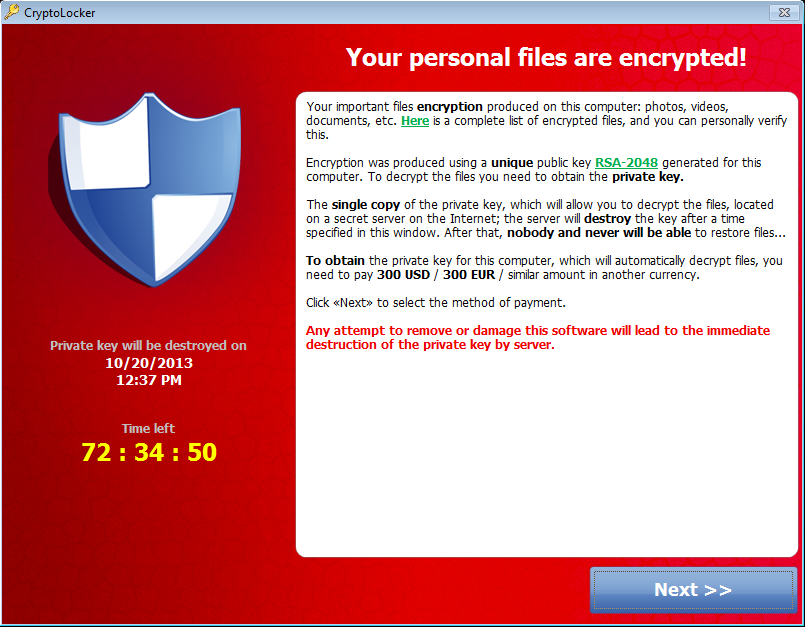
\includegraphics[width=.8\textwidth]{cryptolocker.png}
    \caption{Cryptolocker ransom message.}
    \label{fig:crypto_ransom}
\end{figure}

\paragraph{The Revenues} It is hard to provide a precise estimate of the
earnings that Cryptolocker brought to the attackers. \citeauthor{spagnuolo2013}
\footnote{Michele Spagnuolo is one of the most brilliant persons I have ever had
the chance to know and a friend of mine. Therefore it is a great pleasure of mine to cite
his work.} made a rough estimate of Cryptolocker earnings coming from the
Bitcoin payment system. In total they identified 771 ransoms, for 1,226 BTC (
approximately USD 1,100,000 on December 15, 2013)~\cite{spagnuolo2013}. Such a
measurement was addressed as ``conservative''. It is quite clear that the
Cryptolocker malware is to be considered of a very lucrative threat.


\paragraph{Conclusions} Cryptolocker is a very interesting example of malware
for a few reasons listed here below.
\begin{itemize}
    \item The primary infection vector is via a botnet: The fact that the attackers
        chose this vector lead us to think that in the future most of malware
        will be distributed in such a fashion.
    \item Cryptolocker forms itself a botnet: The network of infected machines
        communicate with the C\&C server in a centralized fashion, employing
        a DGA based rallying scheme.
    \item Being a \emph{ransomware} the malware of the year witnesses the
        attackers' paradigm shift, from no-profit malicious activities carried
        out for hacking interests to profitable ones, capable of massive earnings.
        ``Some men just want to watch the world burn'' is no longer an appropriate
        motto\footnote{The Dark Knight, 2008 Warner Bros.} to address the attackers.
    \item Attackers do not \emph{steal} sensitive personal data, but \emph{lock}
        computer files that, give the majority of targeted extensions, are likely
        to be the result of professionals' work, demonstrating a particular
        attention toward increasing the victims' willingness to pay.
\end{itemize}

All of the aforementioned reasons fully justify the focus of our work, as modern
miscreants' threats leverage the topology and communication scheme we have
tailored our software to search for.

% subsection cryptolocker (end)
% section botnets_a_modern_threat (end)


%-----------------------------------------------------------------------------%
% Summary
%-----------------------------------------------------------------------------%
\section{Summary} % (fold)
\label{sec:summary}
In this section we have introduced the phenomenon of botnets, one of today's most
spread and dangerous threats in computer security. We have briefly overviewed some of
the purposes carried out by these malicious infrastructures. We have explained why most
of these infrastructures feature a \emph{centralized} architecture and employ
a \emph{rallying} mechanism based on Domain Generation Algorithms to establish
the C\&C Channel, the communication medium used to \emph{i)} send orders to
the bots and \emph{ii)} retrieve harvested data or feedback from the bots.
Then we focused on the possible countermeasures to mitigate the threat: Both
sinkholing and takeover do need the C\&C server IP address to be played out.
Finally we have reported two real life cases of botnets in the wild, demonstrating
the threat danger and the actuality.
In the next chapter we focus on the problem we aim at contributing to resolve,
i.e., how to track down a botnet.
% section summary (end)

% chapter botnets (end)